\documentclass[tikz, border=2mm]{standalone}
\usetikzlibrary{positioning, arrows.meta}

\begin{document}
	
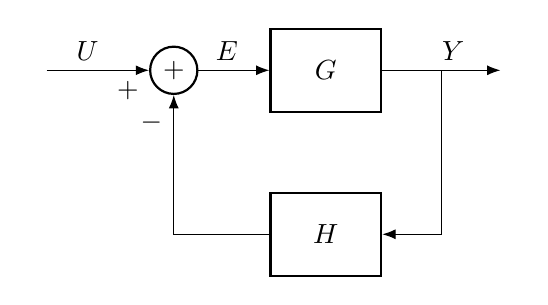
\begin{tikzpicture}[
		block/.style={draw, rectangle, minimum height=3em, minimum width=4em, thick},
		sum/.style={draw, circle, minimum size=6mm, inner sep=0pt, thick},
		node distance=1.2cm and 1.5cm, % Distancia optimizada entre bloques
		>=Latex
		]		
		% --- Camino Directo ---
		% 1. Entrada u
		\node (input) {};
		% 2. Bloques
		\node [sum, right=1.3cm of input] (sum) {+};
		\node [below left=-0.2cm and 0.1cm of sum] {$+$}; % Entrada positiva
		\node [below left=0.2cm and -0.2cm of sum] {$-$};               % Realimentación negativa
		\node [block, right=0.9cm of sum] (blockG) {$G$};
		\node [right=of blockG] (output) {};
		\node [block, below=1cm of blockG] (blockk) {$H$};
%		% Flechas 
		\draw [->] (input) -- node[above, pos=0.4] {$U$}(sum);
		\draw [->] (sum) -- node[above, pos=0.4] {$E$}(blockG);
		\draw [->] (blockG) -- node[above, pos=0.6] {$Y$} (output);		
		% Flechas de realimentación 
		\path (blockG) -- coordinate[pos=0.5] (feedback_node) (output);
		\draw [->] (feedback_node) |- (blockk);
		\draw [->] (blockk) -| (sum);
%		
	\end{tikzpicture}
	
\end{document}